\section{1174008 - Arjun Yuda Firwanda}

\subsection{Teori}
\begin{enumerate}

\item Jelaskan Kenapa Kata-Kata harus dilakukan vektorisasi lengkapi dengan ilustrasi gambar.\par
Karena Vektorisasi merupakan suatu proses konversi data raster menjadi data vektor.

	\begin{figure}[H]
            	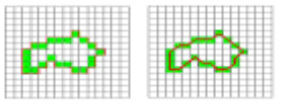
\includegraphics[width=4cm]{figures/1174008/5/vektorisasi.PNG}
           	 \centering
           	 \caption{Vektorisasi}
        	\end{figure}

\item Jelaskan Mengapa dimensi dari vektor dataset google bisa mencapai 300 lengakapi dengan ilustrasi gambar. \par
Karena dimensi vektorisasi akan dijadikan sebagai data training dan data testing. Karena keterbatasan kemampuan komputer yang hanya melakukan train maksimal 300. Sehinggan 80 persen untuk data training dan 20 persen untuk data testing.

	\begin{figure}[H]
		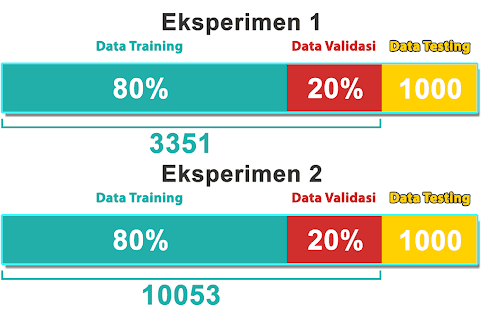
\includegraphics[width=4cm]{figures/1174008/5/vektordataset.PNG}
            	\centering
           	 \caption{Vektorisasi DataSet}
       	 \end{figure}

\item Jelaskan Konsep vektorisasi untuk kata . dilengkapi dengan ilustrasi atau gambar. \par
Konsep vektorisasi digunakan untuk mengukur kemiripan antara suatu dokumen dengan query. Disebut dengan dokumen query, karena query dianggap sebagai vektor-vektor pada ruang n dimensi, dimana n sebagai jumlah seluruh term yang ada di leksikon. Leksikon merupakan daftar term yang ada di indeks.

	\begin{figure}[H]
		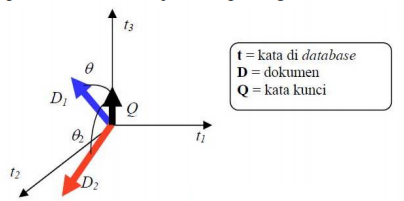
\includegraphics[width=4cm]{figures/1174008/5/vektorisasikata.PNG}
            	\centering
           	 \caption{Vektorisasi Kata}
       	 \end{figure}

\item Jelaskan Konsep vektorisasi untuk dokumen. dilengkapi dengan ilustrasi atau gambar. \par
Vektorisasi dimana data yang terdapat pada file document tersebut diolah dengan melakukan pemrosesan yang mengutamakan nilai data filenamenya atau atribut utama dimana nilai data inputnya tidak terlalu diproses. 

	\begin{figure}[H]
		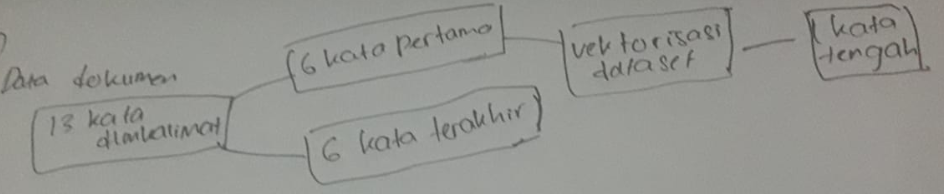
\includegraphics[width=4cm]{figures/1174008/5/vektorisasidokumen.PNG}
            	\centering
           	 \caption{Vektorisasi Dokumen}
       	 \end{figure}

\item Jelaskan apa mean dan standar deviasi, lengkapi dengan iludtrasi atau gambar. \par
Mean adalah nilai rata-rata dari beberapa buah data. Nilai yang terdapat pada mean dapat ditentukan dengan membagi jumlah data dengan banyaknya data. Sedangkan untuk Standar deviasi adalah nilai statistik yang digunakan untuk menentukan bagaimana sebaran data dalam sampel, dan seberapa dekat titik data individu ke mean – atau rata-rata – nilai sampel.

	\begin{figure}[H]
		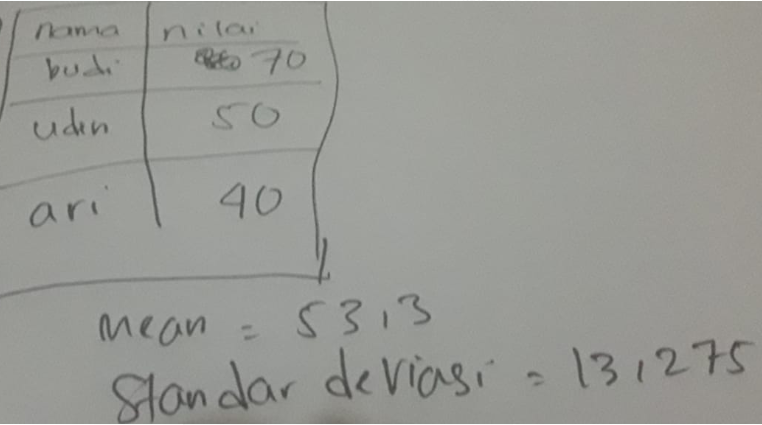
\includegraphics[width=4cm]{figures/1174008/5/meanstandardeviasi.PNG}
            	\centering
           	 \caption{Mean Standard Deviasi}
       	 \end{figure}

\item Jelaskan Apa itu Skip-Gram sertakan contoh ilustrasi. \par
Skip-gram merupakan sebuah teknik yang dapat digunakan di area speech processing, dimana n-gram yang dibentuk kemudian ditambahkan juga dengan tindakan “skip” pada token-tokennya.

	\begin{figure}[H]
		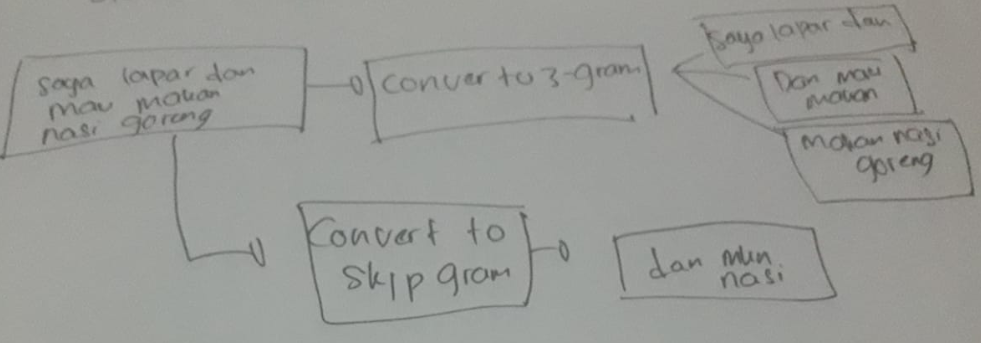
\includegraphics[width=4cm]{figures/1174008/5/skipgram.PNG}
            	\centering
           	 \caption{Skip Gram}
       	 \end{figure}

\end{enumerate}
\subsection{Praktikum}
\begin{enumerate}
\item mencoba dataset google dan penjelasan vektor dari kata love, faith, fall, sick, clear, shine, bag, car, wash, motor, dan cycle.\par

\begin{itemize}
\item berikut merupakan code import gensim digunakan untuk membuat data model atau rangcangan data yang akan di buat. selanjutnya dibuat variabel gmodel yang berisi data vektor negativ. selanjutnya data tersebut di load agar data tersebut dapat di tampilkan dan di olah.

\begin{figure}[ht]
\centering
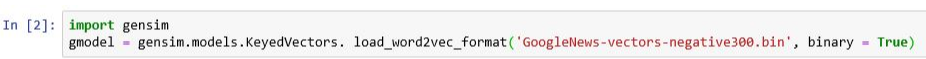
\includegraphics[scale=0.5]{figures/1174008/5/2,1.PNG}
\caption{Praktek 1}
\end{figure}

\item berikut merupakan hasil lpengolahan kata love pada data google yang di load tadi. Sehingga memunculkan hasil vektor 300 dimensi untuk kata tersebut.
\begin{figure}[ht]
\centering
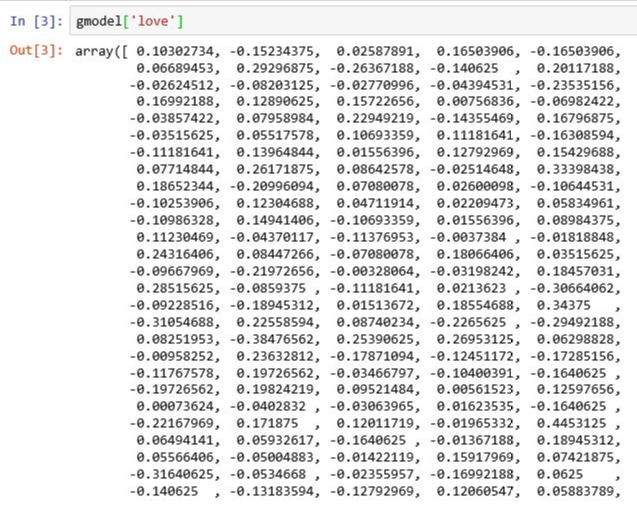
\includegraphics[scale=0.6]{figures/1174008/5/2,1,1.PNG}
\caption{Praktek 1}
\end{figure}

\item berikut merupakan hasil lpengolahan kata faith pada data google yang di load. Sehingga memunculkan hasil vektor 300 dimensi untuk kata tersebut.

\begin{figure}[ht]
\centering
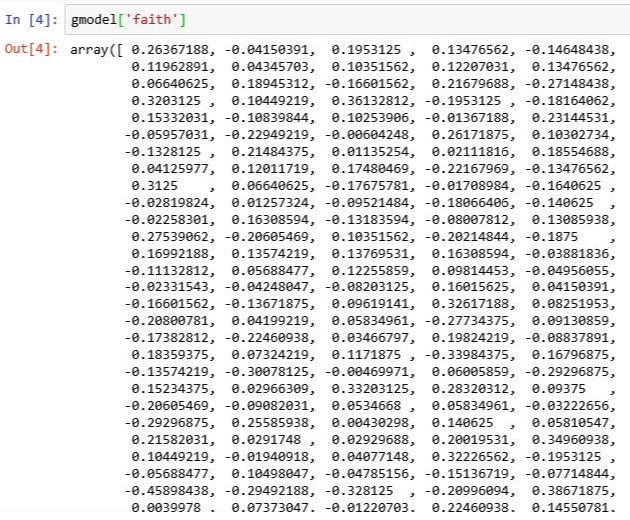
\includegraphics[scale=0.6]{figures/1174008/5/2,1,2.PNG}
\caption{Praktek 1}
\end{figure}

\item berikut merupakan hasil lpengolahan kata fall pada data google yang di load. Sehingga memunculkan hasil vektor 300 dimensi untuk kata tersebut.

\begin{figure}[ht]
\centering
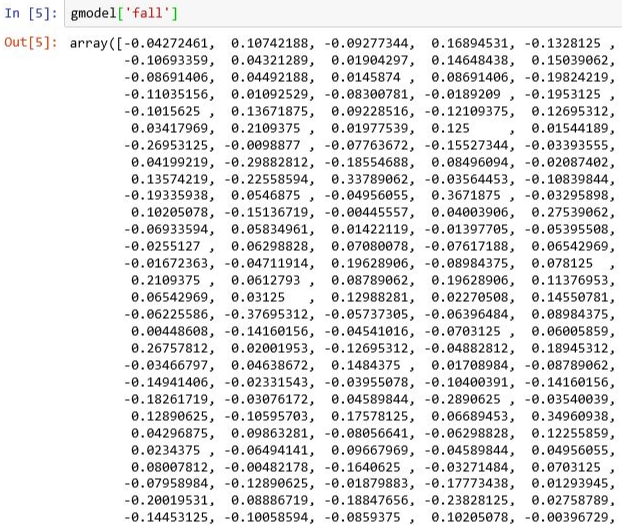
\includegraphics[scale=0.6]{figures/1174008/5/2,1,3.PNG}
\caption{Praktek 1}
\end{figure}

\item berikut merupakan hasil lpengolahan kata sick pada data google yang di load. Sehingga memunculkan hasil vektor 300 dimensi untuk kata tersebut.

\begin{figure}[ht]
\centering
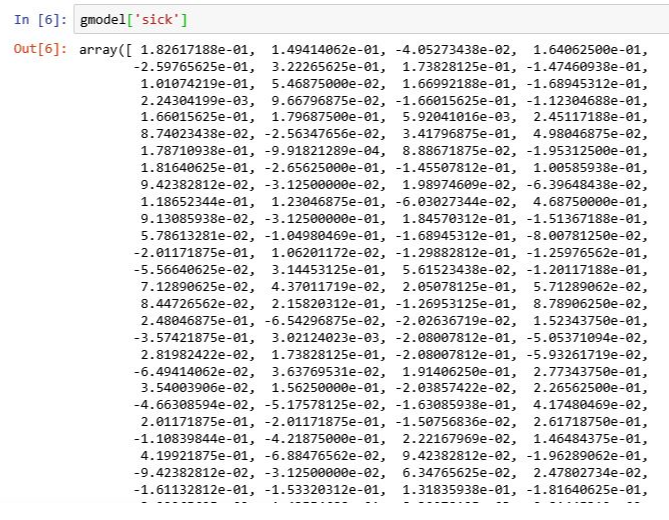
\includegraphics[scale=0.6]{figures/1174008/5/2,1,4.PNG}
\caption{Praktek 1}
\end{figure}


\item berikut merupakan hasil lpengolahan kata clear pada data google yang di load. Sehingga memunculkan hasil vektor 300 dimensi untuk kata tersebut. 

\begin{figure}[ht]
\centering
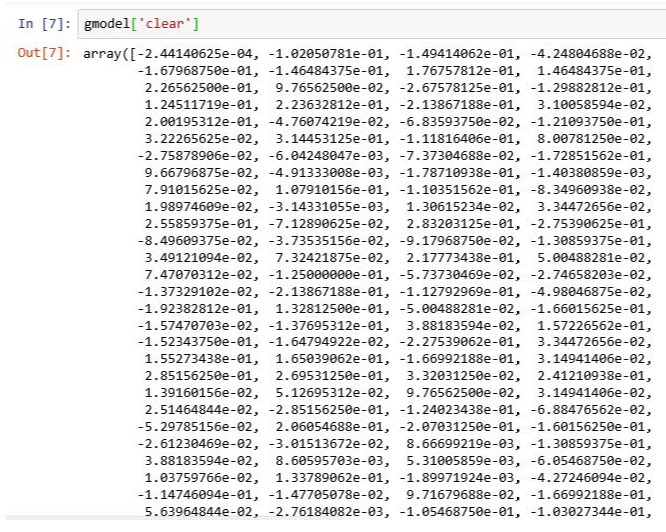
\includegraphics[scale=0.6]{figures/1174008/5/2,1,5.PNG}
\caption{Praktek 1}
\end{figure}

\item berikut merupakan hasil lpengolahan kata shine pada data google yang di load. Sehingga memunculkan hasil vektor 300 dimensi untuk kata tersebut. 

\begin{figure}[ht]
\centering
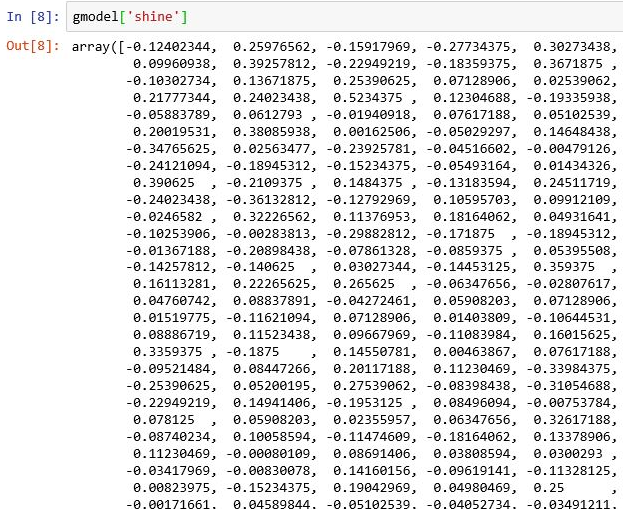
\includegraphics[scale=0.6]{figures/1174008/5/2,1,6.PNG}
\caption{Praktek 1}
\end{figure}

\item berikut merupakan hasil lpengolahan kata bag pada data google yang di load. Sehingga memunculkan hasil vektor 300 dimensi untuk kata tersebut. 

\begin{figure}[ht]
\centering
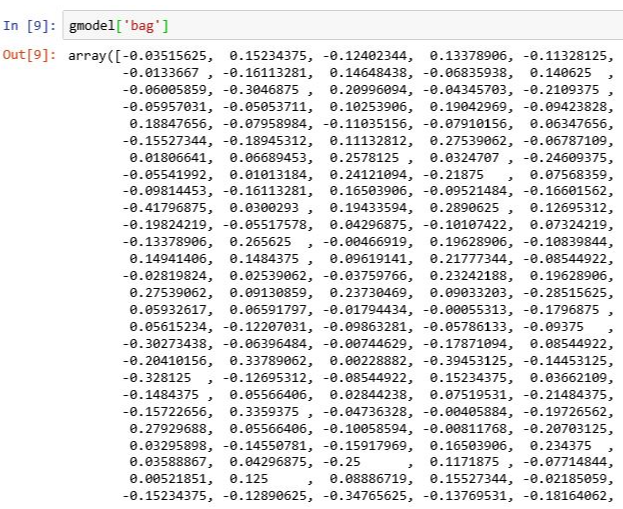
\includegraphics[scale=0.6]{figures/1174008/5/2,1,7.PNG}
\caption{Praktek 1}
\end{figure}

\item berikut merupakan hasil lpengolahan kata car pada data google yang di load. Sehingga memunculkan hasil vektor 300 dimensi untuk kata tersebut. 

\begin{figure}[ht]
\centering
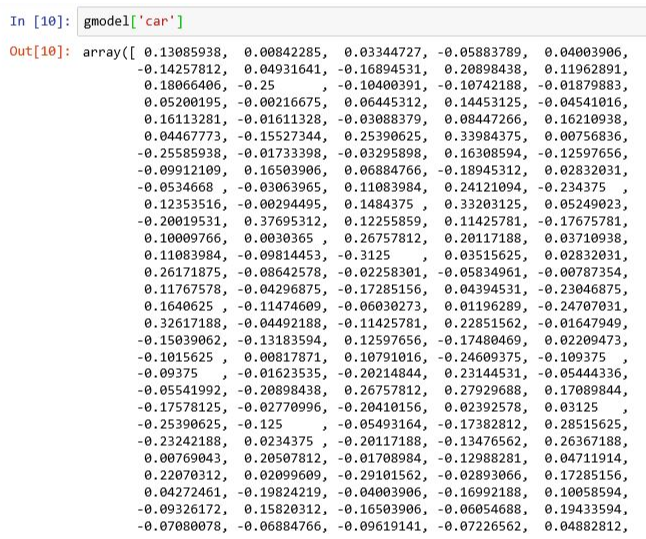
\includegraphics[scale=0.6]{figures/1174008/5/2,1,8.PNG}
\caption{Praktek 1}
\end{figure}

\item berikut merupakan hasil lpengolahan kata wash pada data google yang di load. Sehingga memunculkan hasil vektor 300 dimensi untuk kata tersebut. 

\begin{figure}[ht]
\centering
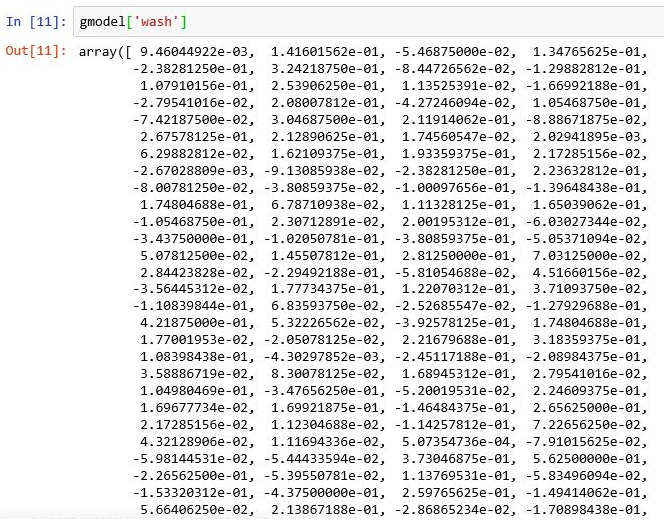
\includegraphics[scale=0.6]{figures/1174008/5/2,1,9.PNG}
\caption{Praktek 1}
\end{figure}

\item berikut merupakan hasil lpengolahan kata motor pada data google yang di load. Sehingga memunculkan hasil vektor 300 dimensi untuk kata tersebut. 

\begin{figure}[ht]
\centering
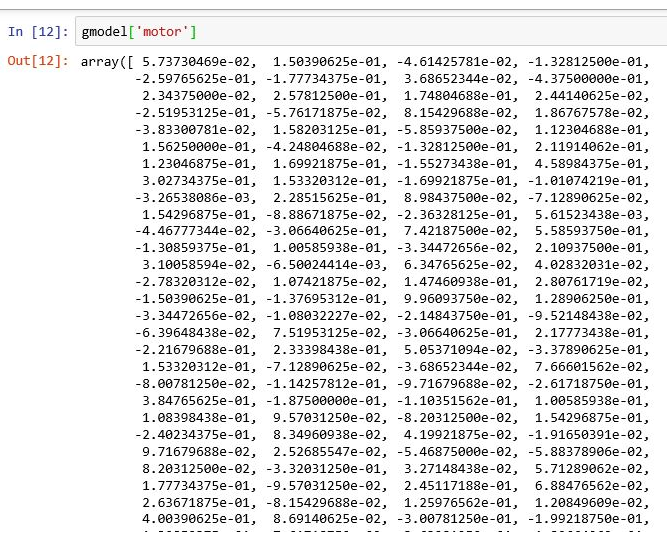
\includegraphics[scale=0.6]{figures/1174008/5/2,1,10.PNG}
\caption{Praktek 1}
\end{figure}

\item berikut merupakan hasil lpengolahan kata cycle pada data google yang di load. Sehingga memunculkan hasil vektor 300 dimensi untuk kata tersebut. 

\begin{figure}[ht]
\centering
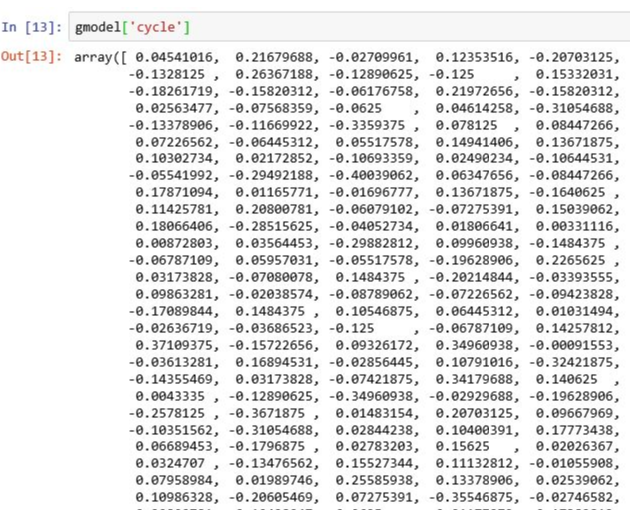
\includegraphics[scale=0.6]{figures/1174008/5/2,1,11.PNG}
\caption{Praktek 1}
\end{figure}

\item berikut merupakan hasil dari similaritas kata kata yang di olah menjadi matrix tadi adapun persentase untuk perbandingan setiap katanya yaitu 9 persen untuk kata wash dan clear 7 persen untuk kata bag dan love 48 persen untuk kata motor dan car 12 persen untuk kata sick dan faith dan terakhir yaitu 6 persen untuk kata cycle dan shine.

\begin{figure}[ht]
\centering
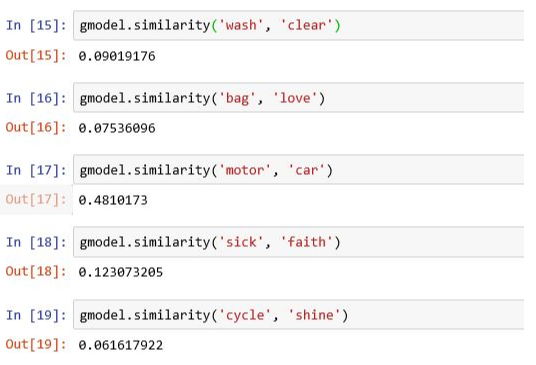
\includegraphics[scale=0.6]{figures/1174008/5/2,1,12.PNG}
\caption{Praktek 1}
\end{figure}

\end{itemize}

\item pada code berikut merupakan hasil dari running code untu ekstrak word dimana pada baris ke tiga dimasukan perintah untuk menghapus tag html yang terdapat dalam file tesebut selanjutnya pada baris ke 4 yaitu perintah untuk menghilangkan tanda kutip satu selanjutnya pada baris ke 5 yaitu perintah untuk menghapus tanda baca pada file tersebut dan yang terakhir yaitu perintah untuk menghapus dable sepasi atau sepasi berurutan. setelah itu dibuat clas bari dari random yang bertujuan untuk mengkocok data yang ada pada file tersebut kemudian class permute sentence tersebut akan di gunkan untuk mengolah data selanjutnya. untuk lebih jelasnya dapat dilihat pada gambar.

\begin{figure}[ht]
\centering
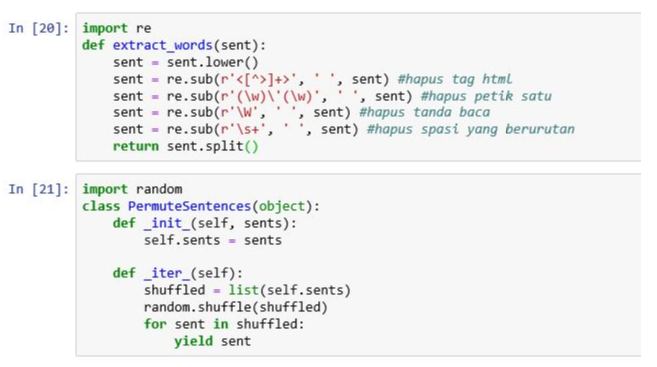
\includegraphics[scale=0.6]{figures/1174008/5/2,2.PNG}
\caption{Praktek 2}
\end{figure}

\item gensim merupakan library untuk memodelkan topik unsuperpise atau memodelkan bahasa dengan model unsuperpise. Sadangkan taget dokumen digunakan untuk TaggetDokumen berarti memasukan dokumen untuk di olah oleh mesin. Kemudian Doc2Vect dugunakan untuk membandingkan dokumen apakah isi dari dokumen itu bobotnya sama dengan dokumen yang di sandingkannya. menunjukan di baris ke satau dilakukan dari librari gensim dokumen mengimport method taggedDocument lalu pada baris kedua dari librari gensim model melakukan import metod Doc2Vec.

\begin{figure}[ht]
\centering
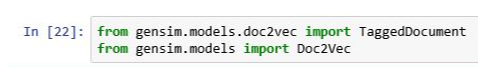
\includegraphics[scale=0.6]{figures/1174008/5/2,3.PNG}
\caption{Praktek 3}
\end{figure}

\item cara memasukan data traning file pertama tentukan terlebih dahulu tempat file dokumen tersebut disimpan kemudian import librari os setelah itu buat variabel unsup\_sentences yang berisikan array kosong, lalu tentukan file yang akan dimasukan setelah itu lakukan os listdir pada data yang akan dimasukan kemudian semua data tersebut di inisialisasi menjadi f kemudian nama f tersebut dimasukan ke variabel unsup. pada codingan tersebut merupakan praktikum untuk memasukan data doc2vec\par

\begin{figure}[ht]
\centering
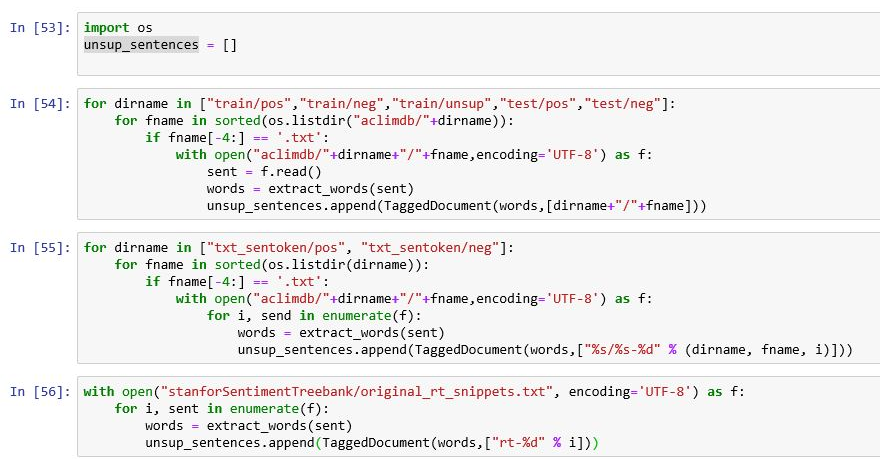
\includegraphics[scale=0.6]{figures/1174008/5/2,4.PNG}
\caption{Praktek 4}
\end{figure}

\item kenapa harus dilakukan pengocokan data atau rendomisasi ? hal ini harus dilakukan supaya data lebis gambang untuk di olah dan meningkatkan tingkat akurasi dari proses pengolahan data Doc2Vec. kemudian harus dilakukan pembersihan data agar memori pc atau laptop yang di gunakan untuk mengolah data menjadi ringan dan menambah peforma dari mesin itu sendiri untuk codingan pertama lakukan terlebih dahulu rendomisasi. selanjutnya membuat variabel baru dengan nama mute yang di isi data class random dan data unsup\_sentence. kemudian setelah pengolahan data dilakukan pembersihan dengan melakukan code.

\begin{figure}[ht]
\centering
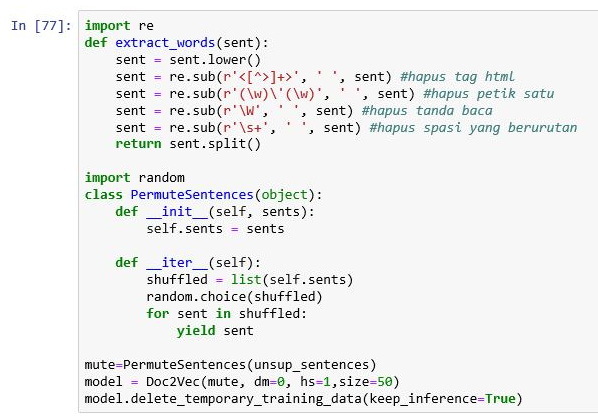
\includegraphics[scale=0.6]{figures/1174008/5/2,5.PNG}
\caption{Praktek 5}
\end{figure}

\item kenapa model harus di save ? suapaya dalam pengolahan data tidak perlu menjalankan kembali data vektorisasi serta untuk meringankan beban ram. kemudian temporary harus dihapus guna meningkatkan peforma komputer.

\begin{figure}[ht]
\centering
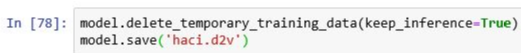
\includegraphics[scale=0.6]{figures/1174008/5/2,6.PNG}
\caption{Praktek 6}
\end{figure}

\begin{figure}[ht]
\centering

\includegraphics[scale=0.6]{figures/1174008/5/2,6,1.PNG}
\caption{Praktek 6}
\end{figure}

\item inver\_code digunakan untuk membandingkan data doc2vec yang telah di olah dengan kata yang baru atau data yang ada dalam perintah vector itu sendiri contoh membandingkan kata (i will go home) untuk lebih jelasnya dapat di lihat pada gambar. kemudian untuk hasil running code tersebut dapat di lihat pada gambar, pada hasil gambar tersebut terdapat hasil vektor yang rata rata berada pada kisaran 0,2 an yang berarti kata yang dimasukan pada inter\_vec datanya ada pada doc2vec atau ada data yang bobotnya menyamai kata-kata di dalam dokumen tersebut.

\begin{figure}[ht]
\centering
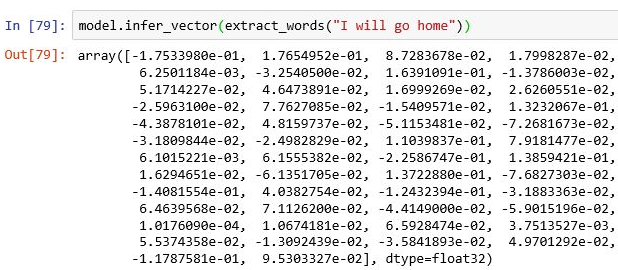
\includegraphics[scale=0.6]{figures/1174008/5/2,7.PNG}
\caption{Praktek 7}
\end{figure}

\item consine\_simirarity setelah melakukan pengolahan data doc2vec dilakukan consine simirarity yang bertujuan untuk membandingkan data berisikan bahasa inggris dengan data yang telah di olah tadi apakah hasilnya mirip atau tidak untuk caranya yaitu dengan cara mencobacodingan yang terdapat pada gambar berikut maka akan muncul hasilnya berapa persen dengan tulisan 0.4 sekian yang berarti tingkat kemiripan dokumen yang di uji tadi untuk hasilnya dapat dilihat pada gambar berikut.

\begin{figure}[ht]
\centering
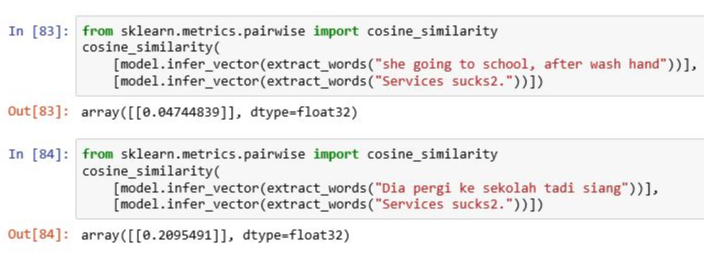
\includegraphics[scale=0.6]{figures/1174008/5/2,8.PNG}
\caption{Praktek 8}
\end{figure}

\item untuk melakukan cross validation pertama masukan terlebih dahulu metode KNeighborsClasifier dan RandomForestClasifier dari library sklearn kemudian dilakukan cross validation setelah itu buat variabel clf dengan isi KNeighborsClasifier dan variabel clfrf dengan isi RandomForestClasifier kemudian di buat skor menggunakan cross validation dengan menggunakan variabel clf dan data sentvecs dan sentiments kemudian dengan numpy dibuat mean dari scores begitu pula untuk variabel clfrf selanjutnya melakukan import metode make\_pipeline yang dilakukan untuk membuat skor dari vektorisasi tfidf dan rf. untuk lebih jelasnya dapat di lihat pada gambar maka akan muncul hasil rata-rata 0,76 sekian atau 76 persen untuk clf yang dapat dilihat pada gambar dan untuk hasil clfrf menghasilkan hasil rata-rata di 71 persen yang dapat dilihat pada gambar dan untuk hasil rata-rata keseluruhan cros validation sebesar 0,74 atau 74 persen yang dapat dilihat pada gambar.

\lstinputlisting{src/1174008/5/2,9.py}

\end{enumerate}

\subsection{Penanganan Error}

\subsection{Bukti Tidak Plagiat}
\begin{figure}[H]
\centering
	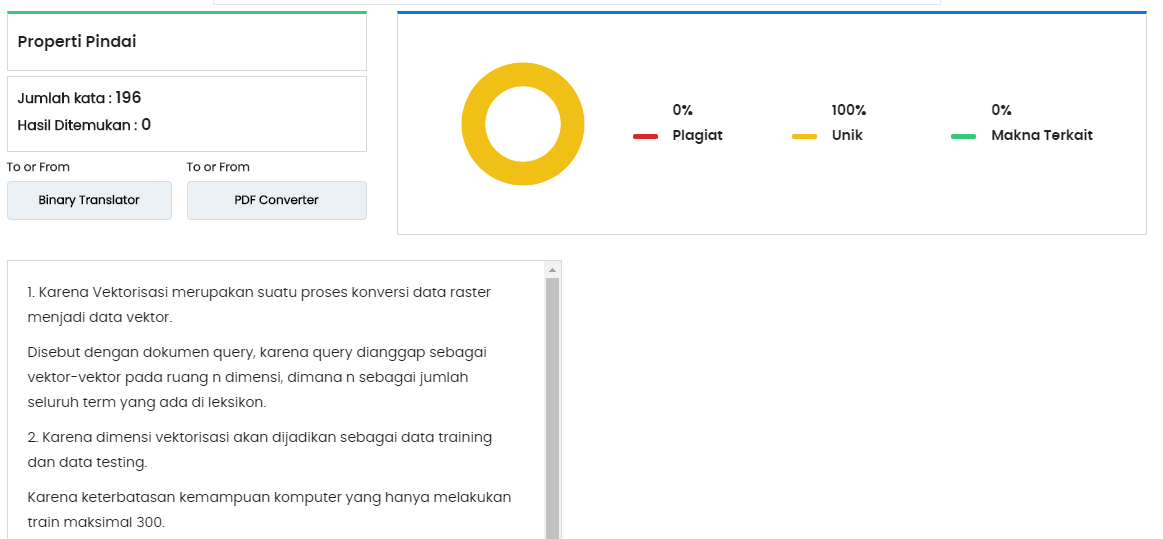
\includegraphics[width=4cm]{figures/1174008/5/bukticekplagiat.PNG}
	\caption{Bukti Tidak Melakukan Plagiat Chapter 5}
\end{figure}
